\subsubsection{Backpropagation}

TODO spomenut hetero-asociativne, jednosmerne, supervised 
TODO not bio-plausible 

The procedure repeatedly adjusts the weights of the connections in the network so as to minimize a measure of the difference between the actual output vector of the net and desired output vector \citet{rumelhart1986learning}. 

The aim is to find a powerful synaptic modification rule that will allow an arbitrarily connected neural network to develop an internal structure that is appropriate for a particular task domain \citet{rumelhart1986learning}. 

Connection within a layer or from higher to lower layers are forbidden, but connections can skip intermediate layers \citet{rumelhart1986learning}.

All units within a layer have their states set in parallel, but different layers have their states set sequentially, starting at the bottom and working upwards until the states of the output units are determined \citet{rumelhart1986learning}. 

$$x_j = \sum_i y_iw_{ji}.$$

$$y_i = \frac{1}{1 + e^{-x_i}}.$$

$$E = \frac{1}{2} \sum_c \sum_j (y_{j,c} - d_{j,c})^2,$$
where $c$ is index over cases. 

To minimize $E$ by gradient descent it is necessary to compute the partial derivate of $E$ with respect to each weight in the network \citet{rumelhart1986learning}. 

$$\partial E / \partial y_j = y_j - d_j.$$

We computed $\partial E / \partial y_j$ for any unit when $\partial E / \partial y_j$ given in the last layer. Repeating this procedure we get $\partial E / \partial y_j$ for all weights. 

Adding momentum:
$\Delta w(t) = -\epsilon \partial E/ \partial w(t) + \alpha \Delta w(t-1).$

Adding a few more connection creates extra dimensions in weight-space and these dimensions provide paths around the barriers that create poor local minima in the lower dimensional subspaces \citet{rumelhart1986learning}. 

The learning procedure, in its current form, is not a plausible model of learning in brains. 

$$\frac{\partial E}{\partial w_{ij}} = -\sum_k(t_k-o_k)w_{jk}\sigma'(\eta_j)s_i,$$
where $t_k$ is the target value, $o_k$ is the output value, $\sigma$ is the nonlinear function, $\eta_j$ is the net input and $s_i$ is the stimulus input \citet{o1996bio}.

%TODO prekreslit do IPE 
\begin{center} 
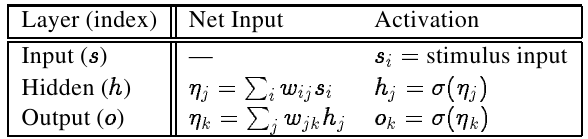
\includegraphics{img/table_bp.png} 
\citet{farkas2013bal} 
\end{center} 
